\chapter{Detecting Anomalous Transactions using KDE}

\section{Designing a custom KDE Class}

The implemented code for the class is:

\begin{lstlisting}[caption={2D Epanechnikov KDE class}]
class EpanechnikovKDE:
    def __init__(self, bandwidth=1.0):
        """Initialize with given bandwidth."""
        self.bandwidth = bandwidth
        self.data = None

    def fit(self, data):
        """Fit the KDE model with the provided data."""
        self.data = np.array(data)

    def epanechnikov_kernel(self, x, xi):
        """Epanechnikov kernel function for 2D using vectorized operations."""
        norm_squared = np.sum(((xi - x) / self.bandwidth) ** 2, axis=-1)
        return ((2 / np.pi) * (1 - norm_squared)) * (norm_squared <= 1)

    def evaluate(self, x):
        """Evaluate the KDE at multiple points x in 2D."""
        return self.epanechnikov_kernel(x, self.data).mean() / (self.bandwidth ** 2)
\end{lstlisting}

\section{Estimating Distribution of Transactions}
For the distribution that is obtained from the given data, we have 2 modes.
The 3D graph for the given data is as follows:

\begin{figure}[H]
  \centering
  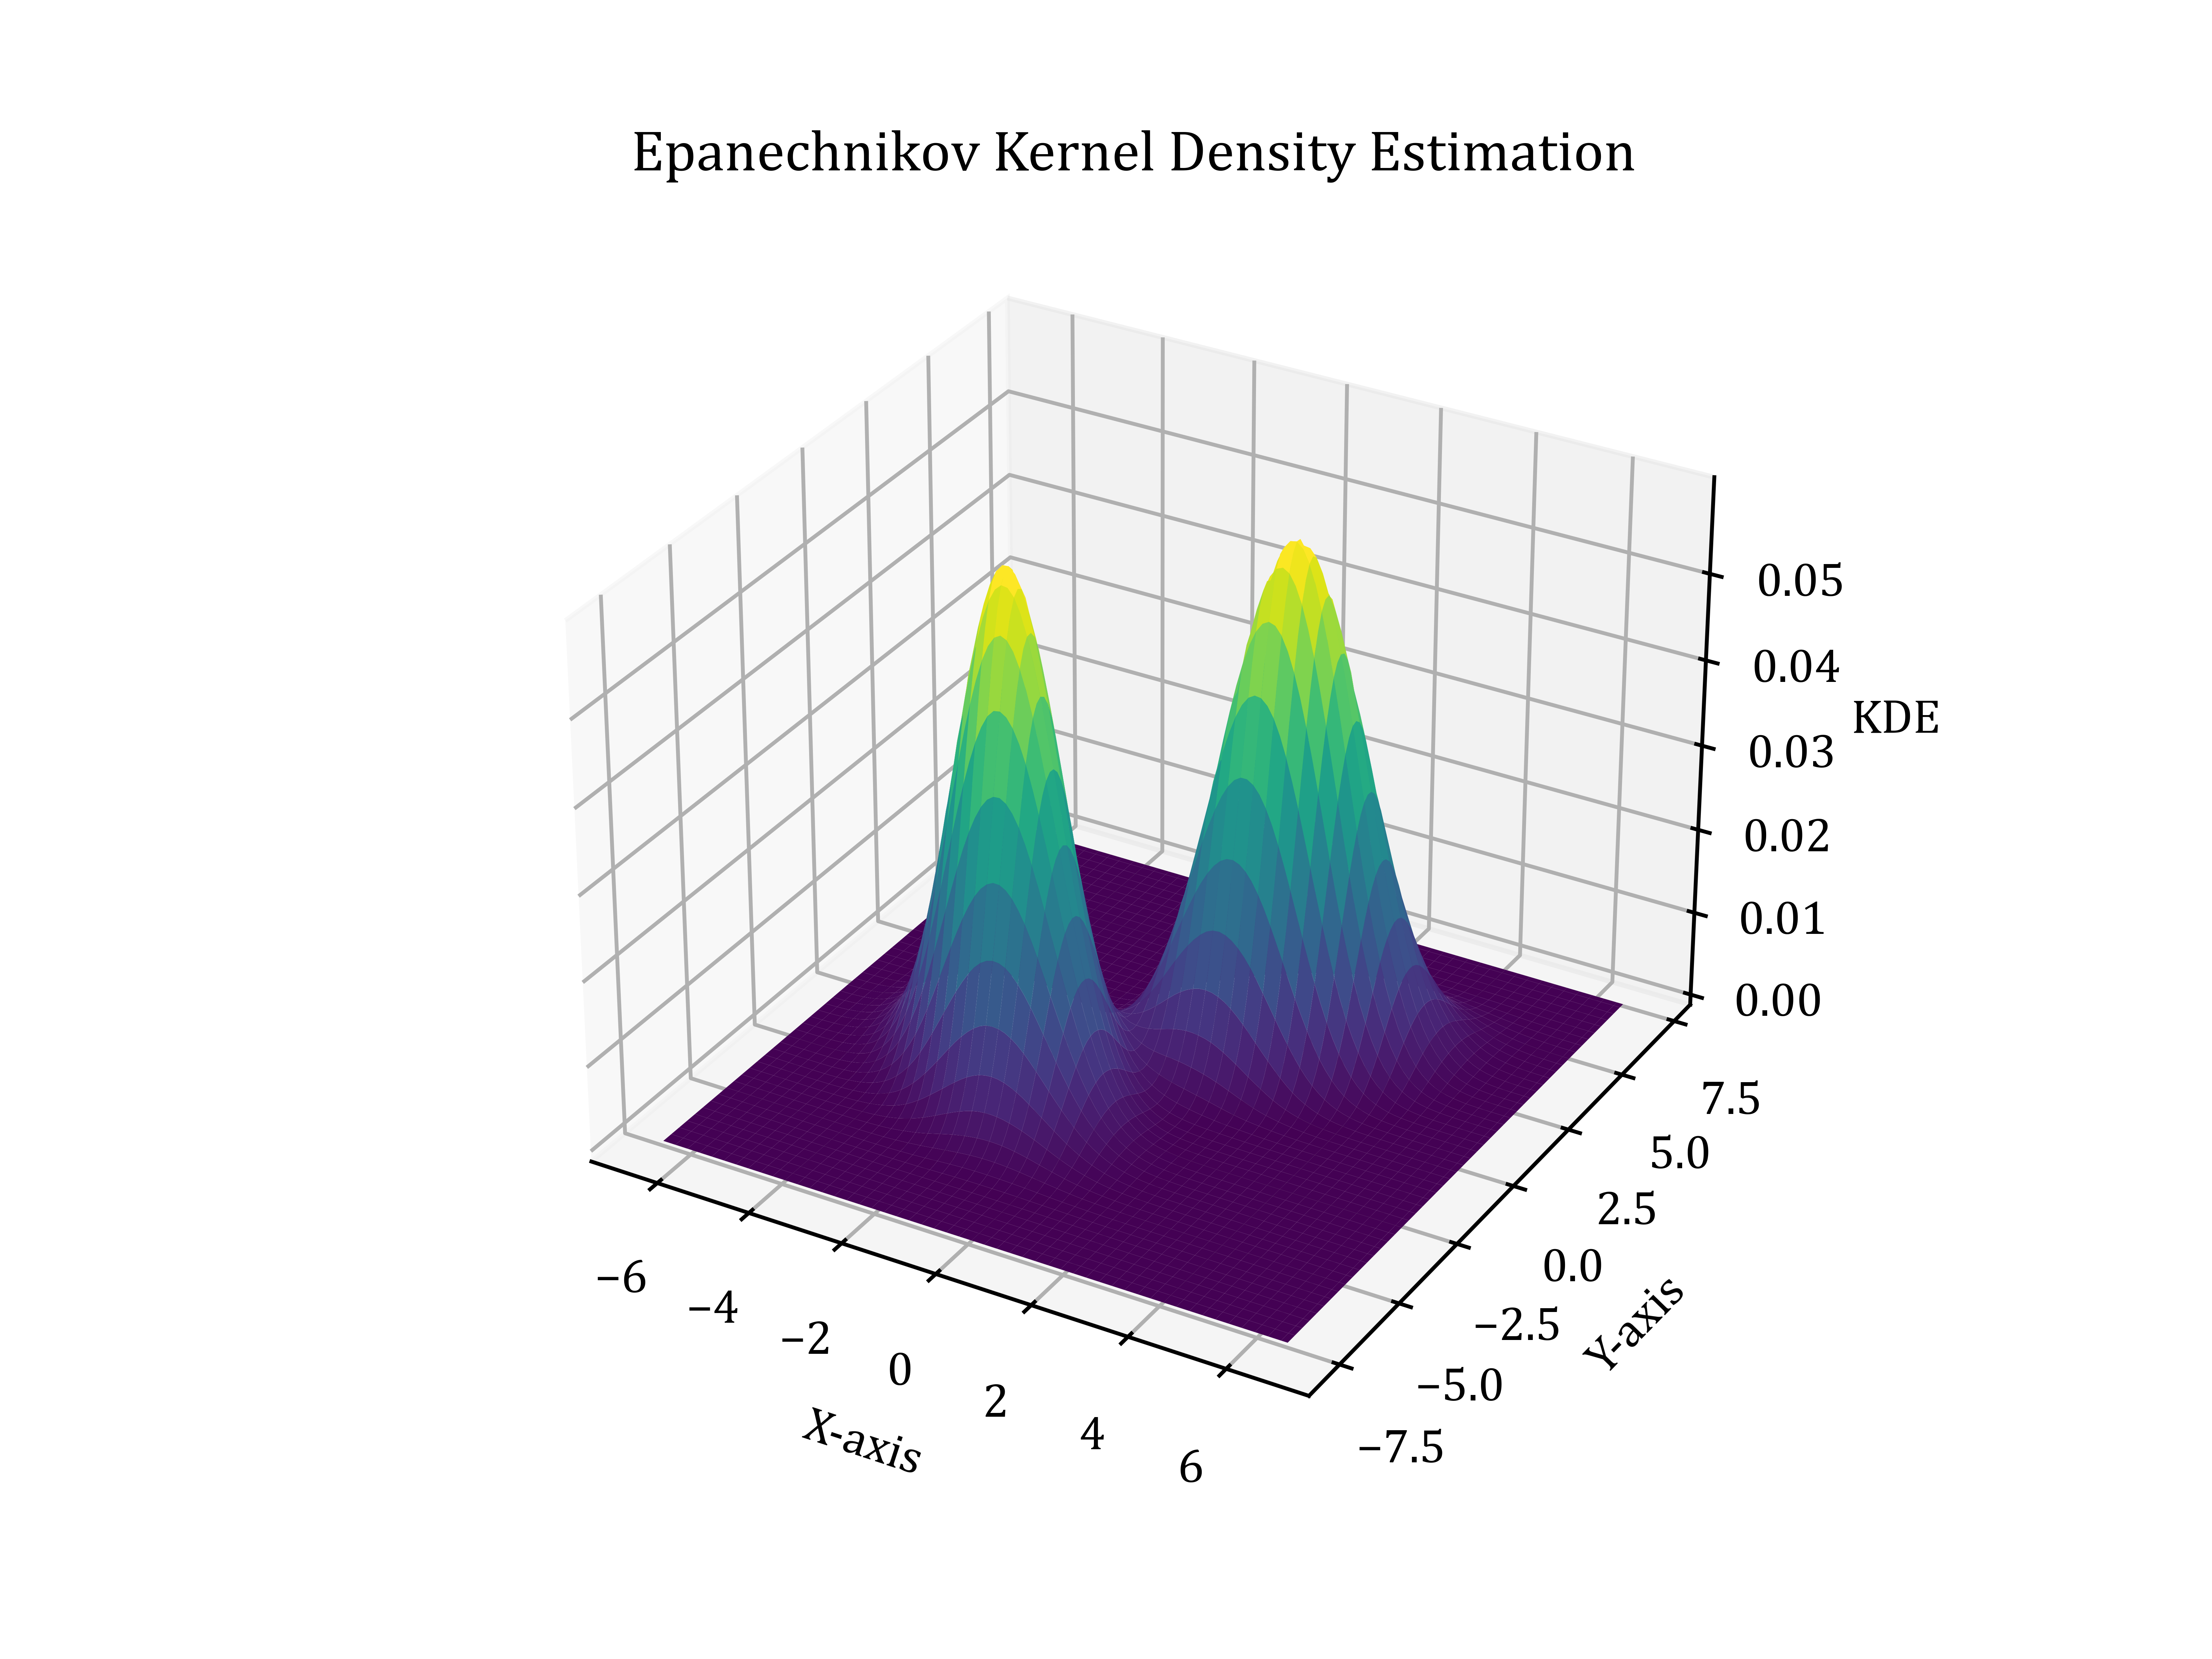
\includegraphics[width=0.4\textwidth]
  {assets/images/transaction_distribution.png}
  \caption{Transaction Distribution}
\end{figure}